\documentclass[smaller,spanish,xcolor=svgnames]{beamer}

% Paquetes personalizados
\usepackage{paquetes} 
\usepackage{colores}
\usepackage{modo}
\usepackage{licencia}
% -------------------------------------------------------------------

\title[Sistemas Expertos]{{\Huge Sistemas Expertos} \\ Diseño de Videojuegos}

\author[Manuel Palomo Duarte - Pablo Recio Quijano - José Tomás Tocino]{Manuel Palomo Duarte \\ Pablo Recio Quijano \\ José Tomás Tocino García}

\date{Junio de 2011}

\begin{document}

\begin{frame}
  \titlepage
\end{frame}

\section{Definiciones}
\subsection{¿Qué es un sistema experto?}
\begin{frame}{¿Qué es un sistema experto?}
  \begin{itemize}
  \item \textbf{Sistema experto:} mecanismo que \textbf{simula} el
    conocimiento de un experto humano en una materia determinada.
  \item Se usan con éxito en muchas ramas de la ciencia: medicina, ingeniería, etc.
  \item Existen varios tipos:
    \begin{itemize}
    \item Basados en \textbf{reglas}. Son los que estudiaremos.
    \item Basados en \textbf{casos}.
    \item Basados en \textbf{redes bayesianas}.
    \end{itemize}
  \end{itemize}
\end{frame}

\subsection{Componentes de un SEBR}
\subsubsection{Componentes principales}

\begin{frame}{Componentes principales}
  \begin{block}{Hechos}
    Información sobre el entorno que el sistema lee y utiliza para tomar
    decisiones.
  \end{block}

  \begin{block}{Reglas}
    Condiciones que el sistema evalúa a partir de los hechos presentes para
    generar nuevo conocimiento.
  \end{block}

  \begin{block}{Motor de inferencia}
    Se encarga de decidir qué reglas pueden activarse según los hechos presentes.
  \end{block}
  
\end{frame}

\subsubsection{Componentes secundarios}

\begin{frame}{Componentes secundarios}
  \begin{block}{Lista de activación (del inglés \textit{agenda})}
    Contiene las reglas cuyas condiciones se han cumplido y son candidatas a
    dispararse.
  \end{block}

  \begin{block}{Estrategias de resolución de conflictos}
    Decide qué regla disparar si hay varias que se cumplen. Puede ser la que más tiempo lleve sin dispararse, la que más veces se halla disparado, una aleatoriamente, etc.
  \end{block}  
\end{frame}

\subsection{Funcionamiento}
\begin{frame}{Funcionamiento}
  \begin{enumerate}
  \item Se leen los hechos.
  \item Se comprueba qué reglas cumplen las condiciones.
  \item Se añaden las reglas candidatas a la agenda.
  \item Se lanzan las reglas de la agenda, generando y/o borrando hechos como resultado de su ejecución.
  \item Vuelta al principio.
  \end{enumerate}
\end{frame}

\begin{frame}{Diagrama de funcionamiento}
  \begin{center}
    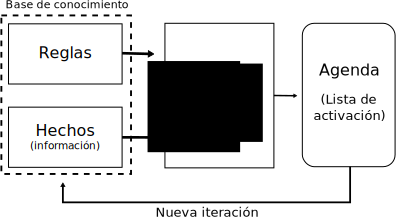
\includegraphics[width=\textwidth]{img/diagrama_funcionamiento}
  \end{center}  
\end{frame}

\section{CLIPS}

\subsection{Introducción}

\begin{frame}{CLIPS}
  \begin{block}{}
    Usaremos \textbf{CLIPS} como sistema para el desarrollo y ejecución de
    sistemas expertos basados en reglas.
  \end{block}

  \begin{itemize}
  \item Es un sistema open source, creado por la NASA y mantenido por uno de sus
    creadores.
  \item Existen muchos wrappers y derivados en otros lenguajes para poder
    interactuar con Clips: Jess (CLIPS para Java), PyCLIPS, FuzzyCLIPS, etc.
  \item Más información en \url{http://clipsrules.sourceforge.net}.
  \end{itemize}
\end{frame}

\subsection{Hechos}

\begin{frame}{Hechos en CLIPS}
  Un \textbf{hecho} en clips tiene la siguiente forma:

  \texttt{(<relación> <campos\_de\_información>)}

  \bigskip

  Por ejemplo:

  \texttt{(persona ``Pepe'')}

  \bigskip

  Se añaden hecho al sistema con \texttt{assert:}

  \texttt{(assert (persona ``Pepe''))}

  \bigskip

  Y se eliminan de él con \texttt{retract}. 

  \texttt{(retract <num\_hecho>)}

  \medskip

  Se puede utilizar \texttt{(facts)} para conocer los hechos y sus números
  asignados.
  
\end{frame}

\begin{frame}[fragile]{Hechos en CLIPS}
  Los \textbf{hechos iniciales} se indican con \texttt{deffacts}:
\begin{verbatim}
(deffacts
 (assert (persona "Pepe" 15))
 (assert (persona "Juan" 18))
 (assert (trabajo "Pepe" "Docente"))
 (assert (trabajo "Juan" "Estudiante"))
)
\end{verbatim}  
\end{frame}

\subsection{Reglas}

\begin{frame}[fragile]{Reglas en CLIPS}
  Las \textbf{reglas} en CLIPS tienen dos partes:
  \begin{enumerate}
  \item \textbf{Condiciones:} serie de hechos y patrones que deben cumplirse
    para que la regla se active.
  \item \textbf{Acciones:} si las condiciones es cumplen, estas acciones se
    lanzarán, normalmente modificando el conjunto de hechos.
  \end{enumerate}

  \bigskip

  Siguen esta sintaxis:
\begin{verbatim}
(defrule <nombre_regla>
  <condiciones>
    =>
  <acciones>
)
\end{verbatim}
\end{frame}

\begin{frame}[fragile]{Reglas en CLIPS}
  Por ejemplo:
\begin{verbatim}
(defrule apagar_fuego
  (hay_emergencia fuego)
   =>
  (assert (llamar bomberos))
)
\end{verbatim}  

  Podemos declarar la prioridad de una regla con \texttt{salience:}

\begin{verbatim}
(defrule <nombre_regla>
  (declare (salience 50))
   ...
\end{verbatim}    
\end{frame}

\begin{frame}[fragile]{Reglas en CLIPS}

  Podemos usar \textbf{condiciones genéricas} que valgan para muchos
  hechos. Por ejemplo, esta regla se ejecutará para todas las personas, guardando
  el nombre de cada persona en la variable \texttt{?n}.

\begin{verbatim}
(defrule imprimir_persona
  (persona ?n)
    =>
  (printout t "Existe una persona cuyo nombre es " 
    ?n crlf)
)
\end{verbatim}
\end{frame}

\begin{frame}[fragile]{Reglas en CLIPS}
  Para hacer \textbf{comprobaciones} arbitrarias, usaremos \texttt{test} con notación infija.

  \medskip

  Es posible guardar \textbf{referencias a hechos} en las condiciones para trabajar con
  ellos en las acciones de la regla:

\begin{verbatim}
(defrule MODULO::jubila1
  (persona ?n ?e)
  ?h <- (trabajo ?n ?t)
  (test (> ?e 65))
    =>
  (retract ?h)
  (assert (jubilado ?n))
)
\end{verbatim}  
\end{frame}

\subsection{Funciones}

\begin{frame}[fragile]{Funciones en CLIPS}
  Podemos modularizar las operaciones en \textbf{funciones} con \texttt{deffunction}. El
  valor de retorno será el de la última expresión evaluada:

\begin{verbatim}
(deffunction MAIN::mayor-mas-uno (?a ?b)
  (if (> ?a ?b) then
    (+ ?a 1)
  else
    (+ ?b 1)
  )
)
\end{verbatim}
\end{frame}

\subsection{Plantillas}

\begin{frame}[fragile]{Plantillas en CLIPS}
  Es posible estructurar la información de un hecho mediante el uso de
  \textbf{plantillas}.

\begin{verbatim}
(deftemplate persona
  (slot nombre)
  (slot edad)
  (slot peso)
)
(assert (persona (nombre "Pepe") (edad 27)))
\end{verbatim}

  Nos permitirá filtrar por campos individuales:

\begin{verbatim}
; Persona de edad 27, da igual el nombre o el peso
?h <- (persona (edad 27))
\end{verbatim}
  
\end{frame}
\section{Gades Siege}

\subsection{Introducción}

\begin{frame}{Introducción}
  \begin{block}{Objetivo}
    Aprender el uso de un sistema experto para la inteligencia artificial \textbf{de un videojuego}, mediante un videojuego ;-)
  \end{block}

  \begin{block}{Idea}
    Crear un sistema para el \textbf{enfrentamiento de dos ejércitos}, cada uno
    controlado por un \textbf{sistema experto} basado en reglas escritas en
    CLIPS por un alumno.
  \end{block}

\end{frame}

\subsection{Planteamiento}

\begin{frame}{Planteamiento}
  \begin{block}{}
    \begin{itemize}
    \item Planteamiento basado en Stratego.
    \item Tenemos un \textbf{tablero} de 8x8, y \textbf{dos ejércitos} de 16 fichas:
      \begin{itemize}
      \item Un \textbf{rey} (valor 1), que cuando muere acaba la partida.
      \item Ocho peones (valor 2).
      \item Dos fichas de valor 3, dos de valor 4 y dos de valor 5.
      \item Una ficha todopoderosa de valor 6.
      \end{itemize}
    \item Por \textbf{turnos}, cada ejército mueve una ficha. Las fichas solo
      pueden moverse una casilla en horizontal o vertical.
    \item Cuando dos fichas \textbf{colisionan}, se muestran sus valores y muere la de
      menor valor, o ambas si hay empate.
    \end{itemize}
  \end{block} 
\end{frame}

\begin{frame}{Historial de versiones}
  El sistema ha evolucionado bastante a lo largo de los años:
  \begin{enumerate}
  \item Versión 0.1, \textbf{modo texto}. Totalmente funcional.
  \item Versión 0.1.1, se añade un \textbf{visor gráfico} para las partidas de texto.
  \item Versión 1.0, \textbf{La Reconquista}, aplicación gráfica e interactiva.
  \item Versión 2.0, \textbf{Resistencia en Cádiz 1812}. Reescritura de la versión 1.0, con
    pruebas automáticas.
  \item Versión 2.x, \textbf{Gades Siege}. Ampliación del proyecto Resistencia 1812,
    mejoras gráficas, nuevas reglas, etc.
  \end{enumerate}  
\end{frame}

\begin{frame}{Versiones}
  \begin{columns}
    \column{0.6\textwidth}
    \begin{block}{Versión 0.1 (Modo texto)}
      \copyright \, Manuel Palomo, 2007\\
      \textit{``Si mi madre me hubiera visto con 8 tíos más gritando y saltando delante de una pantalla negra con letritas, se moría del disgusto''}
    \end{block}
    \column{0.4\textwidth}
    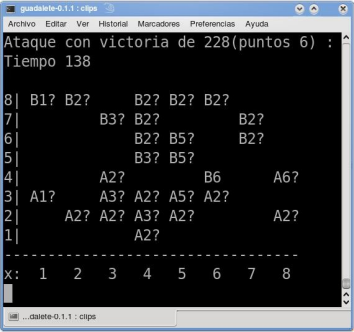
\includegraphics[width=\textwidth]{img/version_1}
  \end{columns}  
\end{frame}

\begin{frame}{Versiones}
  \begin{columns}
    \column{0.6\textwidth}
    \begin{block}{Versión 0.1.1 (Modo texto + Gráfico)}
      \copyright \, Manuel Palomo, Roberto García, 2008\\
      Como alumno colaborador de la asignatura.
    \end{block}
    \column{0.4\textwidth}
    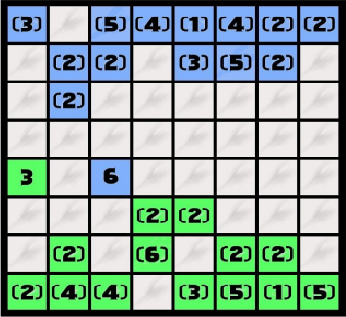
\includegraphics[width=\textwidth]{img/version_2}
  \end{columns}  
\end{frame}

\begin{frame}{Versiones}
  \begin{block}{Versión 1.0 (Aplicación gráfica interactiva)}
      \copyright \, Manuel Palomo, Roberto García, Jesús Soriano, 2009\\
      Proyecto Final de Carrera    
  \end{block}

  \begin{columns}[c]
    \column{0.5\textwidth}
    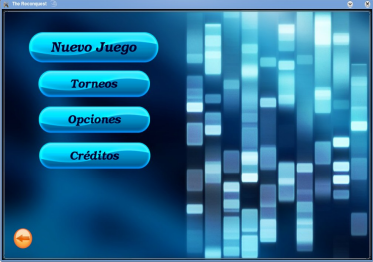
\includegraphics[width=\textwidth]{img/version_31}
    \column{0.5\textwidth}
    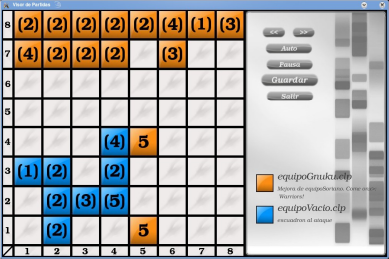
\includegraphics[width=\textwidth]{img/version_32}    
  \end{columns}  
\end{frame}

\begin{frame}{Versiones}
  \begin{block}{Versión 2.0 (Aplicación gráfica interactiva)}
      \copyright \, Manuel Palomo, Pablo Recio, 2010 \\
      Proyecto Final de Carrera    
  \end{block}

  \begin{columns}[c]
    \column{0.5\textwidth}
    \begin{center}
      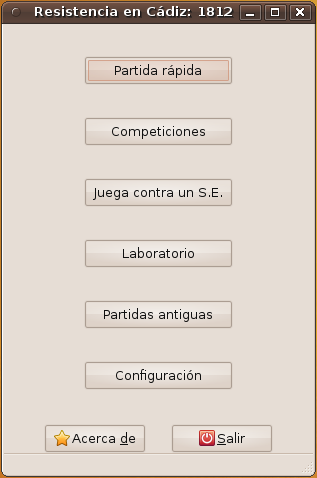
\includegraphics[width=0.5\textwidth]{img/version_41}      
    \end{center}
    \column{0.5\textwidth}
    \begin{center}
      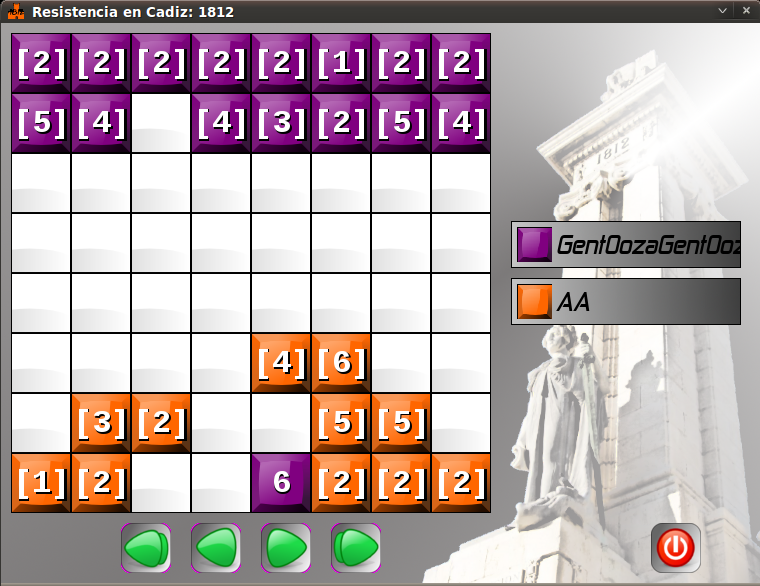
\includegraphics[width=\textwidth]{img/version_42}          
    \end{center}
  \end{columns}  
\end{frame}

\begin{frame}{Versiones}
  \begin{block}{Versión 2.x (Aplicación gráfica interactiva)}
      \copyright \, Manuel Palomo, Pablo Recio, José Tomás Tocino, 2011 \\
      Ampliación y mejora de la versión 2.0
  \end{block}

  \begin{columns}[c]
    \column{0.5\textwidth}
    \begin{center}
      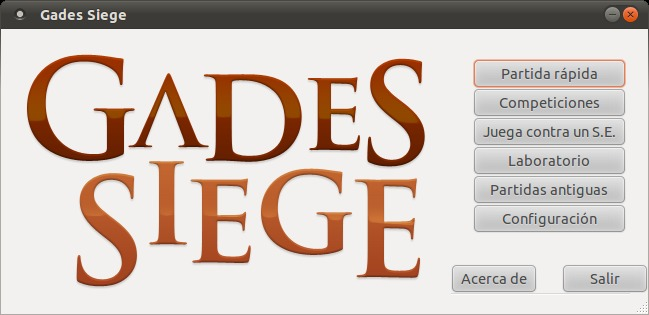
\includegraphics[width=\textwidth]{img/version_51}
    \end{center}

    \column{0.5\textwidth}
    \begin{center}
      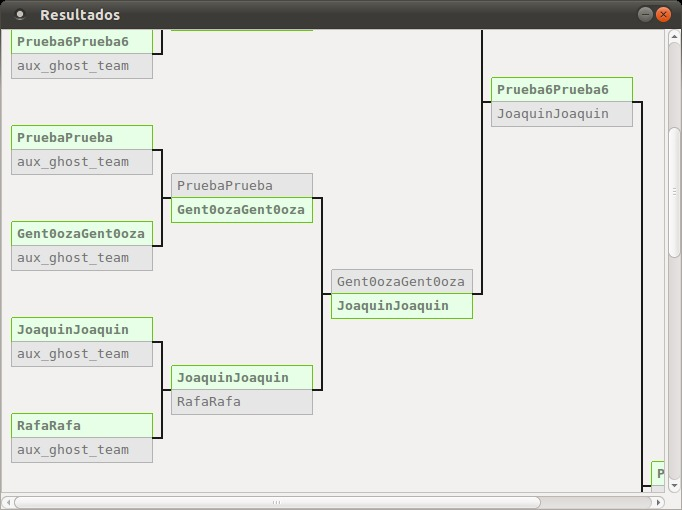
\includegraphics[width=\textwidth]{img/version_52}
    \end{center}

  \end{columns}  
\end{frame}




\subsection{Estructura}

\begin{frame}[fragile]{Estructura del juego: fichas}
  Las \textbf{fichas} en Gades Siege se representan con la plantilla \texttt{ficha}, que
  tiene los siguientes \textit{slots}:
  \begin{description}
  \item[equipo] Puede ser \textit{``A''} (equipo propio) o \textit{``B''} (adversario).
  \item[num] Identificador único de la ficha en el equipo.
  \item[puntos] Valor de la ficha.
  \item[pos-x] Posición horizontal.
  \item[pos-y] Posición vertical.
  \item[descubierta] Valdrá 1 si la ficha está descubierta.
  \end{description}  
\end{frame}


\begin{frame}{Estructura del juego: general}
  \begin{itemize}
  \item El tablero es de 8x8, información que se guarda en un hecho \texttt{(dimension 8)}.
  \item En cada turno, existe un hecho \texttt{(tiempo t)} que indica la
    cantidad de movimientos restantes posibles.
  \item Los equipos de cada jugador se definen en dos ficheros: \texttt{reglasEquipo.clp} y \texttt{equipoEquipo.form}.
  \item El flujo de ejecución es el siguiente:
    \begin{itemize}
    \item Se muestra el estado por pantalla.
    \item Se realiza un movimiento.
    \item Se actualiza el mundo.
    \end{itemize}
  \end{itemize}  
\end{frame}

\begin{frame}[fragile]{Estructura del juego: fichero de formación}
  En el \textbf{fichero de formación} se guardarán las posiciones iniciales de
  las 16 fichas de cada equipo.
  \begin{itemize}
  \item Deben guardarse en la ruta \texttt{data/teams/formations}
  \item Su nombre debe seguir la estructura \texttt{equipoNombre.form}
  \end{itemize}

  \medskip

  Ejemplo de fichero de formación:

\begin{verbatim}
6:5:5:4:4:3:3:2
2:2:2:2:2:2:2:1
\end{verbatim}

  \medskip

  Se colocan los valores de cada ficha en dos filas, tal y como aparecerían en el
  tablero (suponiendo que somos el equipo que juega abajo).
\end{frame}


\begin{frame}[fragile]{Estructura del juego: fichero de reglas}
  En el \textbf{fichero de reglas} se guardarán las reglas que el sistema
  experto usará para jugar.

  \begin{itemize}
  \item Deben guardarse en la ruta \texttt{data/teams/rules}
  \item Su nombre debe seguir la estructura \texttt{reglasNombre.clp}
  \end{itemize}

  \medskip

  En la primera línea del fichero de formación es posible añadir un comentario
  que se verá luego en la interfaz gráfica, siguiendo la siguiente sintaxis:

\begin{verbatim}
; DOC: aquí va el comentario
\end{verbatim}

  \medskip

  De igual modo se pueden añadir comentarios en el resto del fichero usando el
  punto y coma como indicador.
\end{frame}


\begin{frame}[fragile]{Estructura del juego: movimiento}
  En Gades Siege, un \textbf{movimiento} se solitica como un hecho mediante
  una plantilla \texttt{mueve}, que tiene los siguientes \textit{slots}:

  \begin{description}
  \item[num] Identificador de la ficha a mover.
  \item[mov] Número de movimiento.
  \item[tiempo] Momento del tiempo en el que realizar el movimiento.
  \end{description}

  \begin{columns}[c]
    \column{0.5\textwidth}
    {\small
      El número de movimiento responde a la siguiente tabla:
      \begin{itemize}
      \item[1] avanza X
      \item[2] retrocede X
      \item[3] avanza Y
      \item[4] retrocede Y
      \end{itemize}}

    \column{0.5\textwidth}
    \begin{center}
      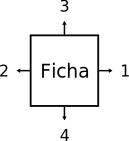
\includegraphics[width=1.2in]{img/diagrama_movimientos}      
    \end{center}

  \end{columns}



\end{frame}

\begin{frame}[fragile]{Estructura del juego: movimiento}
  Por ejemplo, un movimiento horizontal:
\begin{verbatim}
(assert (mueve (num ?n) (mov 1) (tiempo ?t)))
\end{verbatim}

  Las reglas siempre suponen que el jugador empieza en la parte inferior del tablero. si no es así, el sistemas se encarga de traducirlas.
  % Las acciones de las reglas suelen ser asertos de hechos que representan movimientos.
\end{frame}

\begin{frame}[fragile]{Ejemplo de regla 1}
\begin{verbatim}
(defrule EQUIPO-A::atacar1
  (declare (salience 30))
  (ficha (equipo "A") (num ?n1) (pos-x ?x1)
         (pos-y ?y1) (puntos ?p1))
  (ficha (equipo "B") (num ?n2) (pos-x ?x2)
         (pos-y ?y2) (puntos ?p2) (descubierta 1))
  (test (and (> ?p1 ?p2) (= ?y1 ?y2) (> ?x1 ?x2)))
  (tiempo ?t)
    =>
  (assert (mueve (num ?n1) (mov 2) (tiempo ?t)))
)
\end{verbatim}
\end{frame}

\begin{frame}[fragile]{Ejemplo de regla 1, condiciones}

  \small
  \texttt{(defrule EQUIPO-A::atacar1} $\rightarrow$ cabecera de la regla.

  \medskip

  \texttt{(declare (salience 30))} $\rightarrow$ declaramos la prioridad de la regla.

  \medskip

  \texttt{(ficha (equipo ''A'') (num ?n1) (pos-x ?x1) (pos-y ?y1) (puntos ?p1))} $\rightarrow$ buscamos una ficha cualquiera de nuestro equipo, guardando su posición y puntos.

  \medskip

  \texttt{(ficha (equipo "B") (num ?n2) (pos-x ?x2) (pos-y ?y2) (puntos ?p2) (descubierta 1))} $\rightarrow$ buscamos una ficha adversaria, que esté descubierta.

  \medskip

  \texttt{(test (and (> ?p1 ?p2) (= ?y1 ?y2) (> ?x1 ?x2)))} $\rightarrow$ comprobamos que:
  \begin{itemize}
  \item Nuestra ficha sea superior a la otra ficha.
  \item Ambas fichas estén en la misma columna (igual \texttt{pos-y}).
  \item Nuestra ficha esté más a la derecha que la otra ficha.
  \end{itemize}

  \medskip

  \texttt{(tiempo ?t)} $\rightarrow$ guardamos el turno en la variable t.
\end{frame}

\begin{frame}{Ejemplo de regla 1, acciones}
  Si todas las condiciones anteriores se cumplen, esto es, se han encontrado
  fichas que cumplan los criterios indicados, se ejecutan las acciones.

  \medskip

  \texttt{(assert (mueve (num ?n1) (mov 2) (tiempo ?t)))}

  \medskip

  Mueve nuestra ficha en la dirección de la ficha adversaria (con intención de capturarla).
\end{frame}


\begin{frame}[fragile]{Ejemplo de regla 2}
\begin{verbatim}
(defrule EQUIPO-A::atacar2
  (declare (salience 20))
  (ficha (equipo "A") (num ?n1) (pos-x ?x1)
         (puntos ?p1))
  (ficha (equipo "B") (num ?n2) (pos-x ?x2)
         (puntos ?p2) (descubierta 1))
  (test (and (> ?p1 ?p2) (> ?x1 ?x2)))
  (tiempo ?t)
    =>
  (assert (mueve (num ?n1) (mov 2) (tiempo ?t)))
)
\end{verbatim}
\end{frame}

\begin{frame}[fragile]{Ejemplo de regla 3}
\begin{verbatim}
(defrule EQUIPO-A::huir1
  (declare (salience 20))
  (ficha (equipo "A") (num ?n1) (pos-x ?x1)
         (pos-y ?y1) (puntos 1))
  (ficha (equipo "B") (pos-x ?x2) (pos-y ?y2)
         (puntos 5))
  (test (and (= ?x1 ?x2) (> ?y1 ?y2)))
  (tiempo ?t)
   =>
  (assert (mueve (num ?n1) (mov 4) (tiempo ?t)))
)
\end{verbatim}
\end{frame}

\begin{frame}[fragile]{Ejemplo de regla 4}
\begin{verbatim}
(defrule EQUIPO-A::despistar
  (declare (salience 10))
  (ficha (equipo "A") (num 11) (pos-x ?x1)
         (pos-y ?y1))
  (test (< ?y1 4))
  (not (ficha (equipo "A") (pos-x ?x1)
              (pos-y (+ 1 ?y1))))
  (tiempo ?t)
    =>
  (assert (mueve (num 11) (mov 3) (tiempo ?t)))
)
\end{verbatim}
\end{frame}

\begin{frame}{¡A trabajar!}
  \begin{itemize}
  \item Intentad crear reglas \textit{inteligentes} y valientes.
  \item Disponéis de prioridades entre 1 (mínima) y 80 (máxima).
  \item Se pueden usar funciones.
  \item No podéis modificar los hechos de tiempo, dimensión y fichas.
  \item Se pueden usar hechos auxiliares si se desea.
  \item Existen reglas con prioridad 0 que se disparan si no hay ninguna
    mejor. Éstas hacen oscilar las fichas entre (4,4) y (5,5).
  \item Más información en \url{http://gsiege.googlecode.com}
  \end{itemize}
\end{frame}

\licencia

\end{document}







